\documentclass[11pt]{article}
\usepackage{geometry,marginnote} % Pour passer au format A4
\geometry{hmargin=1cm, vmargin=1.5cm} % 

% Page et encodage
\usepackage[T1]{fontenc} % Use 8-bit encoding that has 256 glyphs
\usepackage[english,french]{babel} % Français et anglais
\usepackage[utf8]{inputenc} 

\usepackage{lmodern}
\usepackage[np]{numprint}
\setlength\parindent{0pt}

% Graphiques
\usepackage{graphicx,float,grffile}
\usepackage{tikz,pst-eucl,pst-plot,pstricks,pst-node,pstricks-add,pst-fun,pgfplots} 

% Maths et divers
\usepackage{amsmath,amsfonts,amssymb,amsthm,verbatim,scratch3}
\usepackage{multicol,enumitem,url,eurosym,gensymb,tabularx}

\DeclareUnicodeCharacter{20AC}{\euro}



% Sections
\usepackage{sectsty} % Allows customizing section commands
\allsectionsfont{\centering \normalfont\scshape}

% Tête et pied de page
\usepackage{fancyhdr} \pagestyle{fancy} \fancyhead{} \fancyfoot{}

%\fancyfoot[L]{Collège Faubert}
%\fancyfoot[C]{\thepage / 6}
%\fancyfoot[R]{Série Générale}

\renewcommand{\headrulewidth}{0pt} % Remove header underlines
%\renewcommand{\footrulewidth}{0pt} % Remove footer underlines

\newcommand{\horrule}[1]{\rule{\linewidth}{#1}} % Create horizontal rule command with 1 argument of height

\newcommand{\Pointilles}[1][3]{%
  \multido{}{#1}{\makebox[\linewidth]{\dotfill}\\[\parskip]
}}

\newtheorem{Definition}{Définition}

\usepackage{siunitx}
\sisetup{
    detect-all,
    output-decimal-marker={,},
    group-minimum-digits = 3,
    group-separator={~},
    number-unit-separator={~},
    inter-unit-product={~}
}

\setlength{\columnseprule}{1pt}


\begin{document}

\begin{center}
  \textit{Il faut apprendre, non pas pour l'amour de la connaissance, mais pour se défendre contre le mépris dans lequel le monde tient les ignorants.} - \textbf{Charlie Chaplin}
\end{center}

\textbf{DEF1} \\

Donner la définition de l'inégalité triangulaire.\\

\textbf{ex1 - Démontrer} \\

Peut-on construire un triangle à partir de ces trois longueurs.

\begin{itemize}[label={$\bullet$}]
  \item Triangle 1 : $126cm$ , $134cm$  et $214cm$.
  \item Triangle 2 : $541cm$ , $253cm$ et $128cm$.
  \item Triangle 3 : $167cm$ , $241cm$ et $132cm$.
\end{itemize} 

\textbf{ex2 - Calculer} \\

Donner l'ensemble des longueurs possibles permettant au triangle d'exister. 

\begin{itemize}[label={$\bullet$}]
  \item $126cm$ et $134cm$.
  \item $541cm$ et $253cm$.
  \item $167cm$ et $241cm$.
\end{itemize}

\textbf{pb1 : Entretien BMW} \\

\begin{multicols}{2}

La révision des 4 ans ou 60 000km comporte : 

\begin{itemize}[label={$\bullet$}]
  \item Filtre à air : 130€
  \item Filtre à carburant : 115€
  \item Bougies : 85€ 
  \item Services huile moteur 45€
  \item Microfiltres d'habitacle 15€  
\end{itemize} 

Calculer le prix de la révision. \columnbreak

\begin{figure}[H]
  \centering
  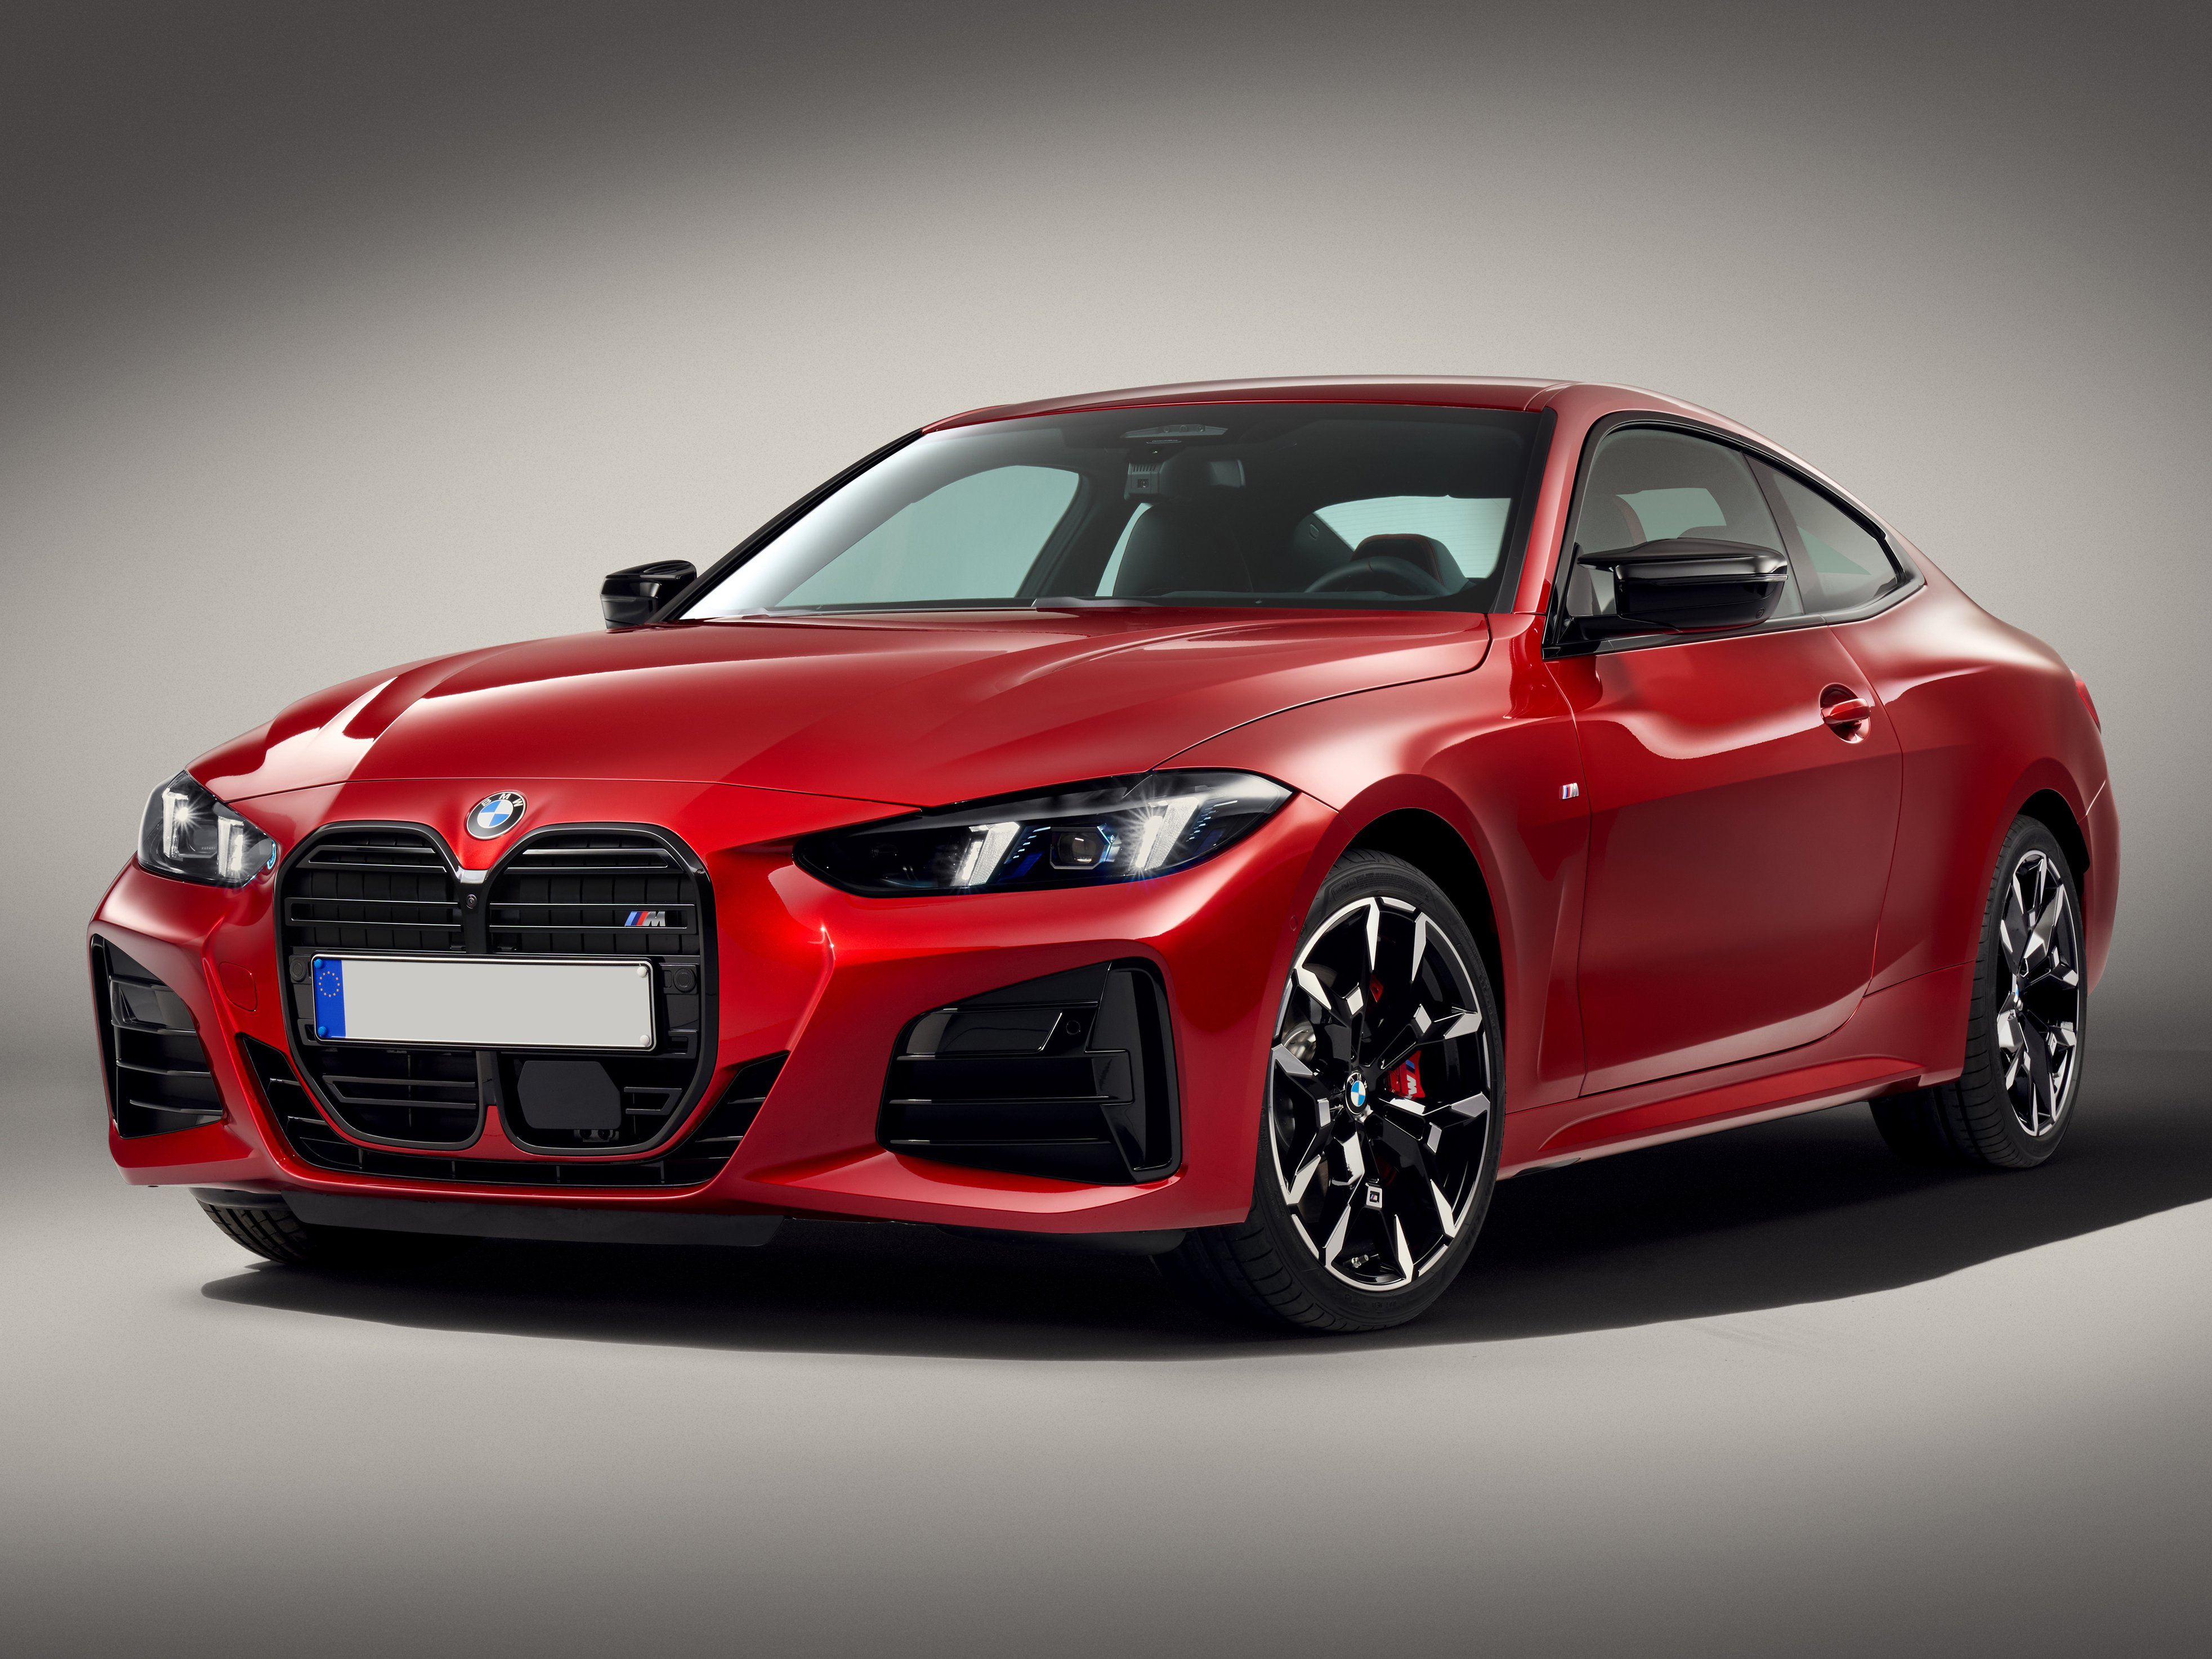
\includegraphics[width=0.6\linewidth]{5x2-inegalite-triangulaire/bmw.jpg}
\end{figure}

\end{multicols}

\textbf{pb2 : Réalisation d'un covering sur une Lamborghini} \\

\begin{multicols}{2} 

\begin{figure}[H]
  \centering
  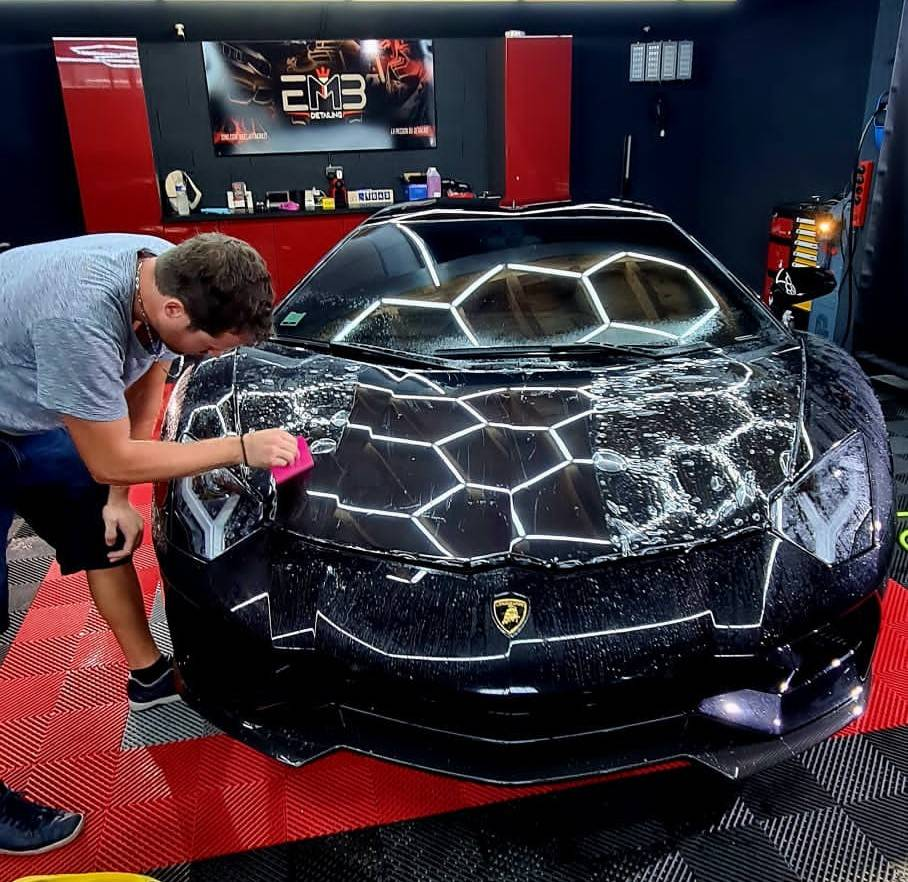
\includegraphics[width=0.6\linewidth]{5x2-inegalite-triangulaire/lambo.jpg}
\end{figure} \columnbreak

\textit{Le covering est une spécialité de préparation automobile visant à appliquer un film de décoration ou de protection sur l'ensemble de la voiture.} \\

Un carrossier spécialise en covering facture l'opération 4\,200€ pour une Lamborghini . Le client souhaite un covering de décoration DBZ.
Pour réaliser ce covering, le carrossier doit acheter le film de décoration 2\,800€. Il compte 6h pour poser le film de décoration correctement. \\

Quel est son bénéfice ? 

\end{multicols}

\newpage

\textbf{pb3 : Entretien des roues et du freinage sur une Porsche} \\

\begin{multicols}{2} 

Lewis Hamilton souhaite faire du circuit avec sa Porsche 911. Mais avant d'enchaîner les tours de piste, il souhaite changer les 4 pneus ainsi que les 4 plaquettes de frein. \\

Il hésite entre deux offres : 

\begin{itemize}[label={$\bullet$}]
  \item Naruto : 1 roue et 1 plaquette neuves pour 64€.
  \item Midas : 2 roues neuves pour 75€ et 2 plaquettes pour 56€. 
\end{itemize} \columnbreak

\begin{figure}[H]
  \centering
  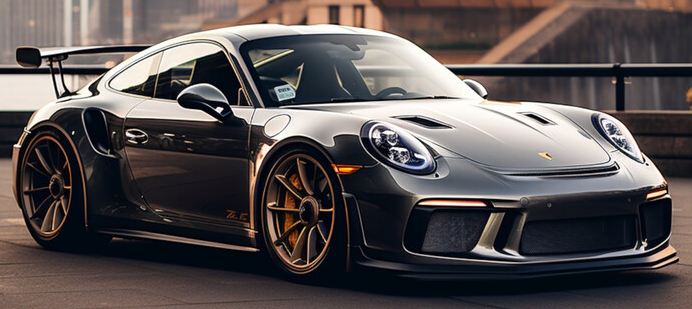
\includegraphics[width=0.9\linewidth]{5x2-inegalite-triangulaire/porsche.png}
\end{figure} 
\end{multicols}

Quelle est l'offre la plus avantageuse ?\\

\textbf{pb4 : Pit Stop F1} \\

\begin{multicols}{2} 

\begin{figure}[H]
  \centering
  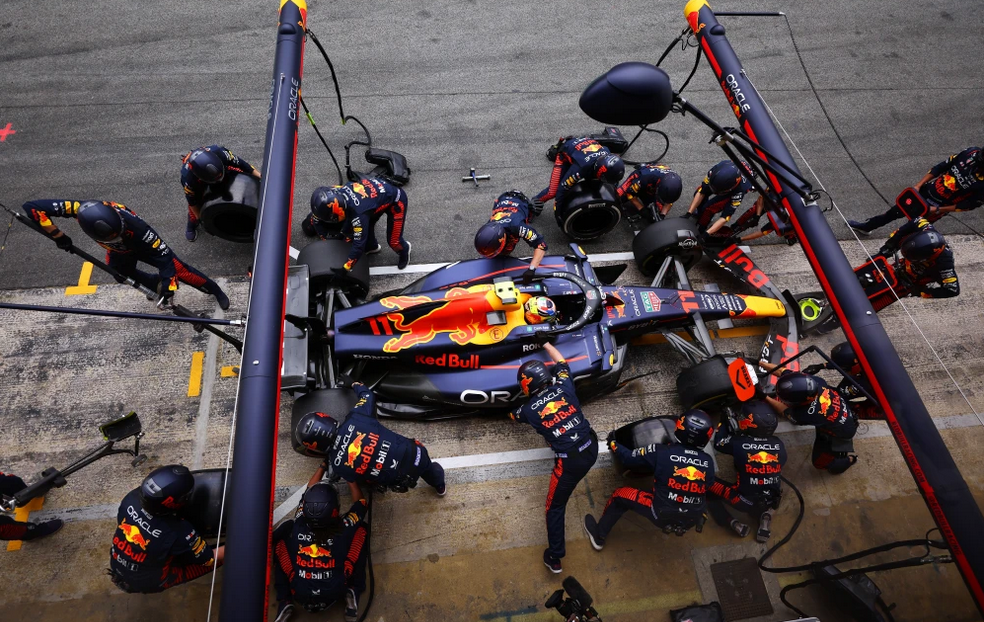
\includegraphics[width=0.8\linewidth]{5x2-inegalite-triangulaire/f1.png}
\end{figure}  \columnbreak

Dans une course de Formule 1, 22 mécaniciens vont en même temps s'occuper de changer les roues, mettre du carburant et réaliser diverses petites actions importantes. Les meilleurs équipes arrivent à changer les 4 pneus autour des 2,2 secondes en général. \\

L'équipe Red Bull réalise un excellent temps de 2 secondes pour le Pit Stop. Cela permet au pilote Max Verstappen de gagner la course et de monter sur la première marche du podium. Il gagne une prime de 51\,000€. Il garde 12\,000€ pour lui et souhaite que l'équipe de mécaniciens se partage équitablement le reste. \\
\end{multicols}


Quelle somme d'argent va recevoir chaque mécanicien de l'équipe Red Bull ?\\

\textbf{pb5 : Mon vélo} \\

\begin{figure}[H]
  \centering
  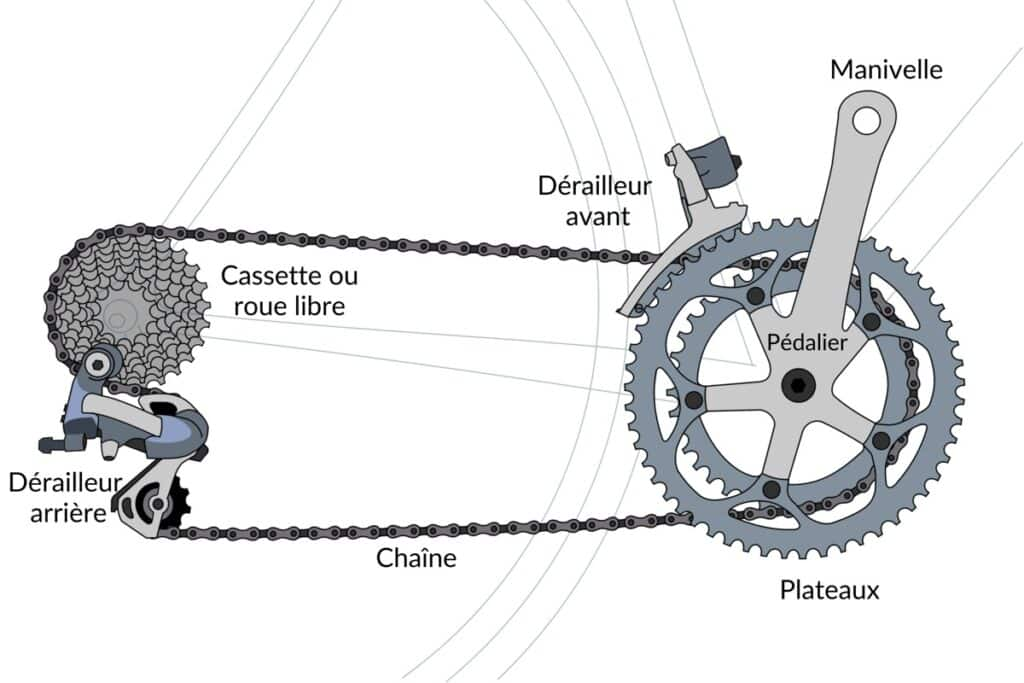
\includegraphics[width=0.4\linewidth]{5x2-inegalite-triangulaire/velo.jpg}
\end{figure} 

Soyons réaliste, vous avez plus de chance de croiser votre professeur en vélo. Équipé d'un rutilant VTT Décath et de gros mollets, il grimpe la côte en petit plateau et grand pignon. Quand il réalise un tour entier avec le pédalier, la roue arrière fait un quart de tour. Il compte 126 tours de pédalier. 

\begin{enumerate}
  \item[1.] Combien de tours la roue a-t-elle effectué ?
  \item[2.] La roue a un rayon de 60cm. Calculer la distance parcourue. \\
    Rappel : Longueur du contour d'un cercle : $P = 2 \times \Pi \times Rayon$.   
\end{enumerate}

\newpage


\begin{center}
  \textit{Il faut apprendre, non pas pour l'amour de la connaissance, mais pour se défendre contre le mépris dans lequel le monde tient les ignorants.} - \textbf{Charlie Chaplin}
\end{center}

\textbf{DEF1} \\

Donner la définition de l'inégalité triangulaire.\\

\textbf{ex1 - Démontrer} \\

Peut-on construire un triangle à partir de ces trois longueurs.

\begin{itemize}[label={$\bullet$}]
  \item Triangle 1 : $186cm$ , $134cm$  et $114cm$.
  \item Triangle 2 : $341cm$ , $653cm$ et $128cm$.
  \item Triangle 3 : $154cm$ , $241cm$ et $432cm$.
\end{itemize} 

\textbf{ex2 - Calculer} \\

Donner l'ensemble des longueurs possibles permettant au triangle d'exister. 

\begin{itemize}[label={$\bullet$}]
  \item $186cm$ et $134cm$.
  \item $341cm$ et $653cm$.
  \item $154cm$ et $241cm$.
\end{itemize}

\textbf{pb1 : Entretien BMW} \\

\begin{multicols}{2}

La révision des 4 ans ou 60 000km comporte : 

\begin{itemize}[label={$\bullet$}]
  \item Filtre à air : 120€
  \item Filtre à carburant : 135€
  \item Bougies : 75€ 
  \item Services huile moteur 55€
  \item Microfiltres d'habitacle 12€  
\end{itemize} 

Calculer le prix de la révision. \columnbreak

\begin{figure}[H]
  \centering
  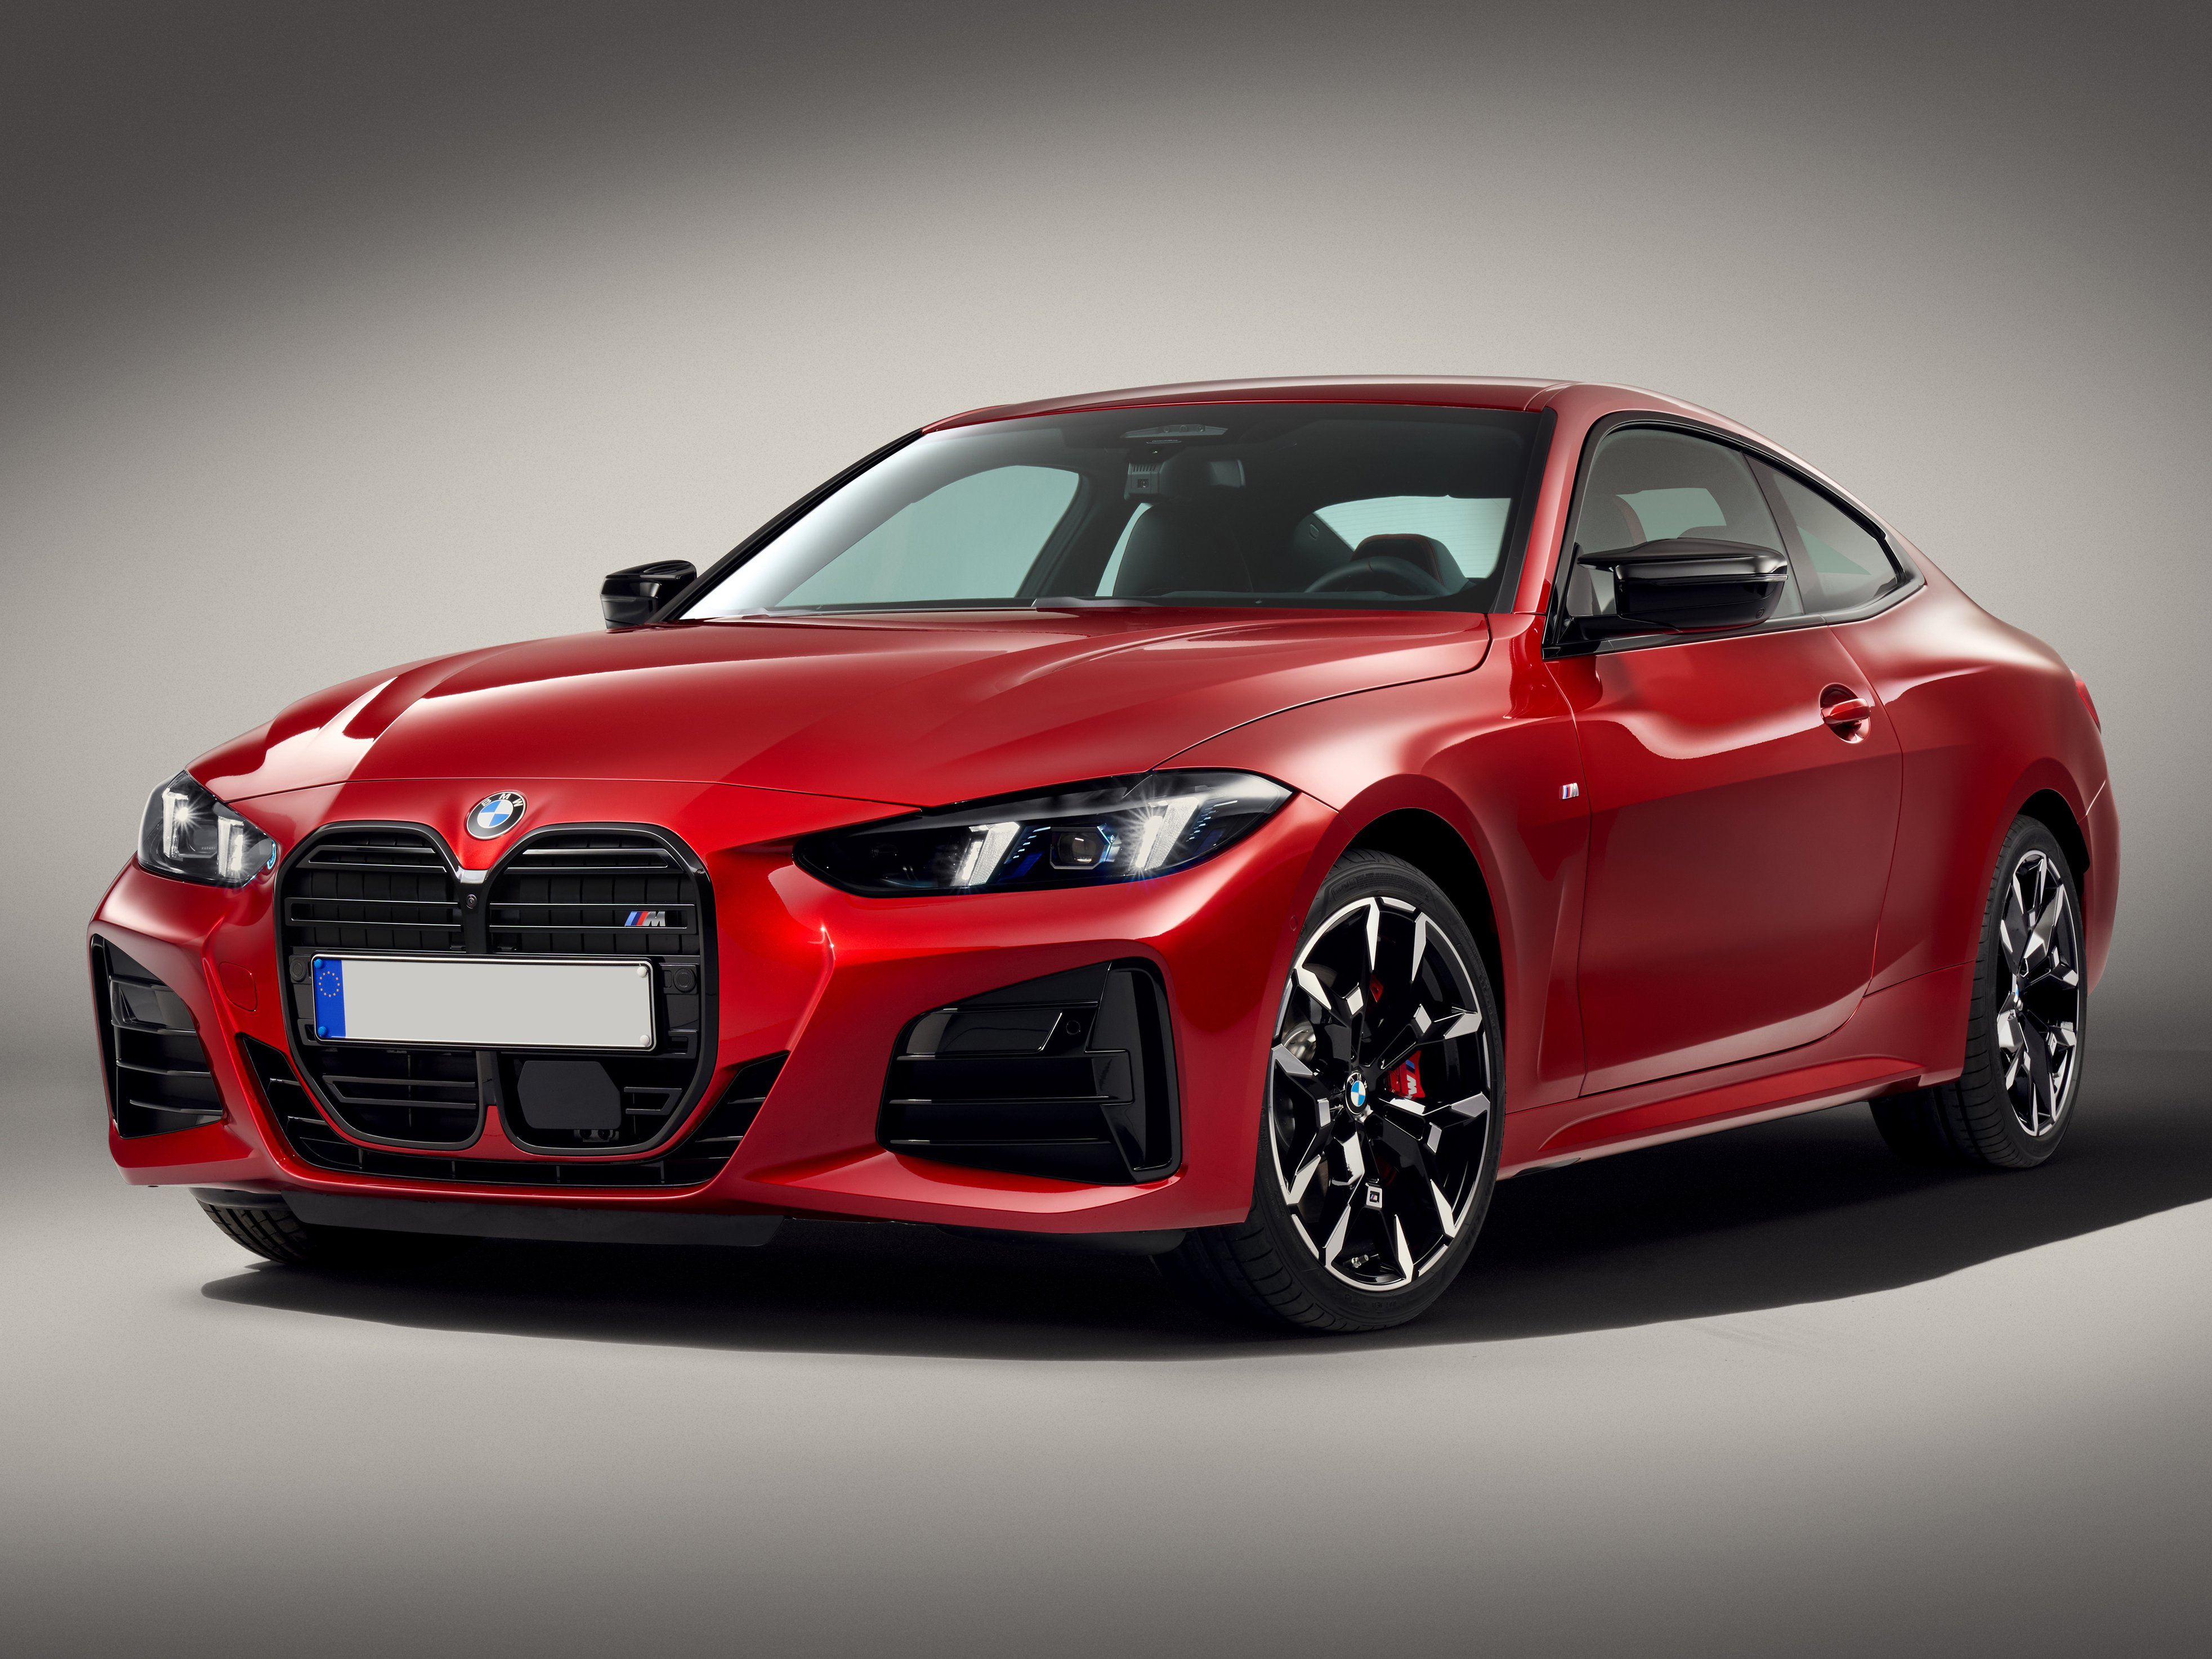
\includegraphics[width=0.6\linewidth]{5x2-inegalite-triangulaire/bmw.jpg}
\end{figure}

\end{multicols}

\textbf{pb2 : Réalisation d'un covering sur une Lamborghini} \\

\begin{multicols}{2} 

\begin{figure}[H]
  \centering
  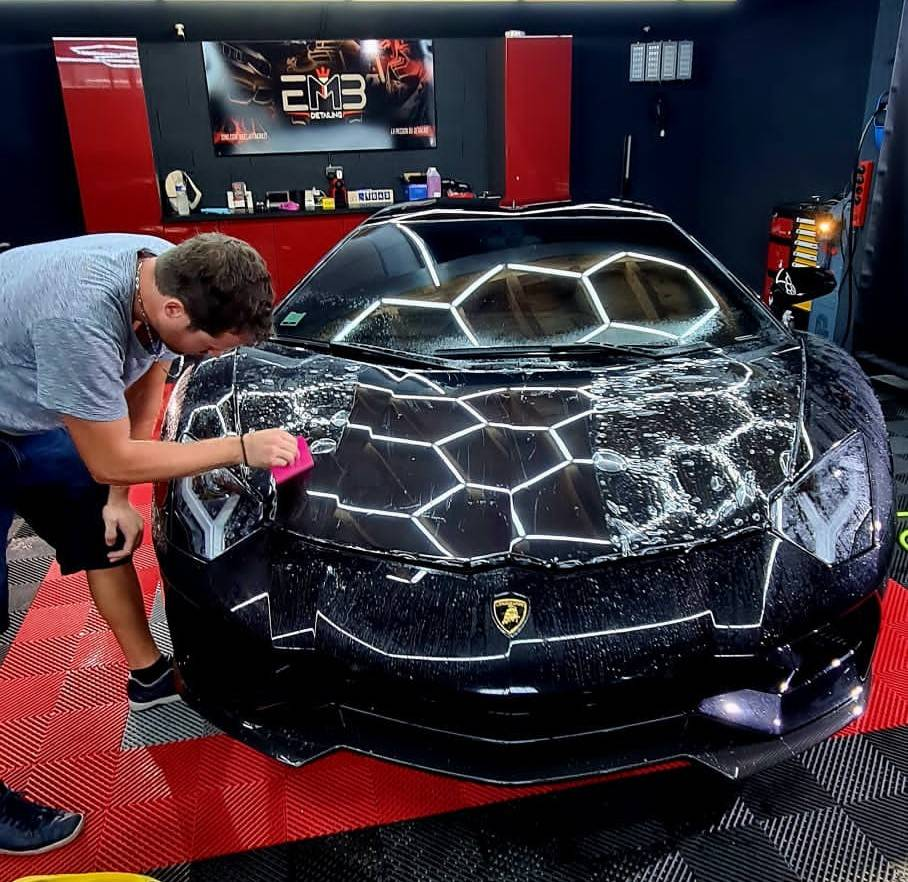
\includegraphics[width=0.6\linewidth]{5x2-inegalite-triangulaire/lambo.jpg}
\end{figure} \columnbreak

\textit{Le covering est une spécialité de préparation automobile visant à appliquer un film de décoration ou de protection sur l'ensemble de la voiture.} \\

Un carrossier spécialise en covering facture l'opération 4\,600€ pour une Lamborghini . Le client souhaite un covering de décoration DBZ.
Pour réaliser ce covering, le carrossier doit acheter le film de décoration 2\,900€. Il compte 6h pour poser le film de décoration correctement. \\

Quel est son bénéfice ? 

\end{multicols}

\newpage

\textbf{pb3 : Entretien des roues et du freinage sur une Porsche} \\

\begin{multicols}{2} 

Lewis Hamilton souhaite faire du circuit avec sa Porsche 911. Mais avant d'enchaîner les tours de piste, il souhaite changer les 4 pneus ainsi que les 4 plaquettes de frein. \\

Il hésite entre deux offres : 

\begin{itemize}[label={$\bullet$}]
  \item Naruto : 1 roue et 1 plaquette neuves pour 68€.
  \item Midas : 2 roues neuves pour 75€ et 2 plaquettes pour 56€. 
\end{itemize} \columnbreak

\begin{figure}[H]
  \centering
  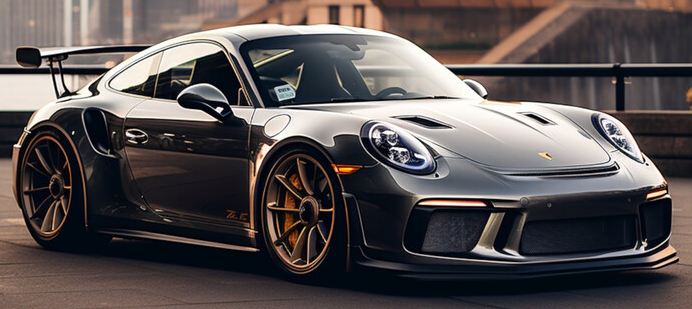
\includegraphics[width=0.9\linewidth]{5x2-inegalite-triangulaire/porsche.png}
\end{figure} 
\end{multicols}

Quelle est l'offre la plus avantageuse ?\\

\textbf{pb4 : Pit Stop F1} \\

\begin{multicols}{2} 

\begin{figure}[H]
  \centering
  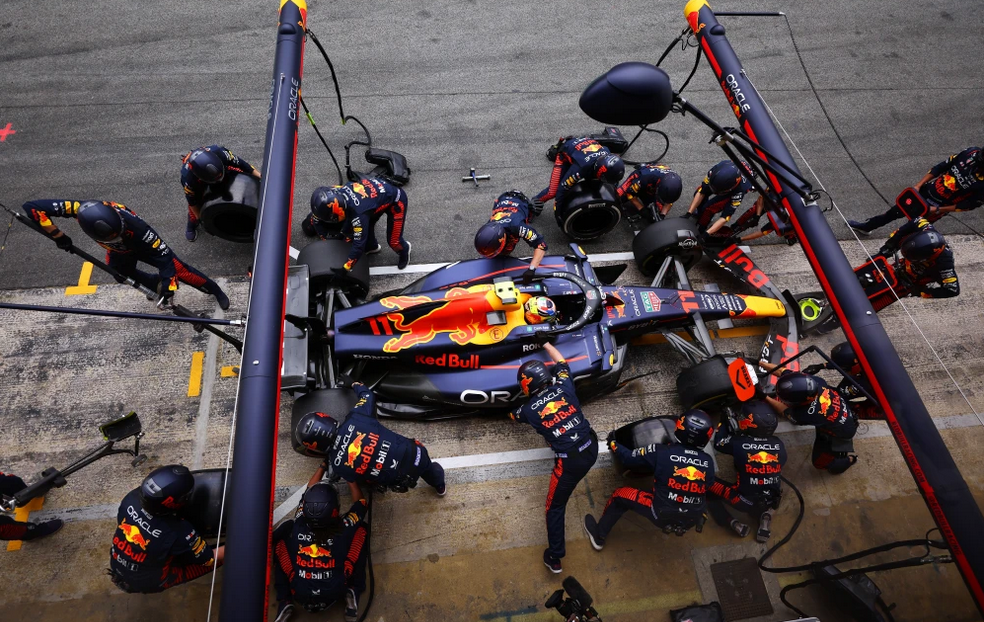
\includegraphics[width=0.8\linewidth]{5x2-inegalite-triangulaire/f1.png}
\end{figure}  \columnbreak

Dans une course de Formule 1, 22 mécaniciens vont en même temps s'occuper de changer les roues, mettre du carburant et réaliser diverses petites actions importantes. Les meilleurs équipes arrivent à changer les 4 pneus autour des 2,2 secondes en général. \\

L'équipe Red Bull réalise un excellent temps de 2 secondes pour le Pit Stop. Cela permet au pilote Max Verstappen de gagner la course et de monter sur la première marche du podium. Il gagne une prime de 61\,000€. Il garde 21\,000€ pour lui et souhaite que l'équipe de mécaniciens se partage équitablement le reste. \\
\end{multicols}


Quelle somme d'argent va recevoir chaque mécanicien de l'équipe Red Bull ?\\

\textbf{pb5 : Mon vélo} \\

\begin{figure}[H]
  \centering
  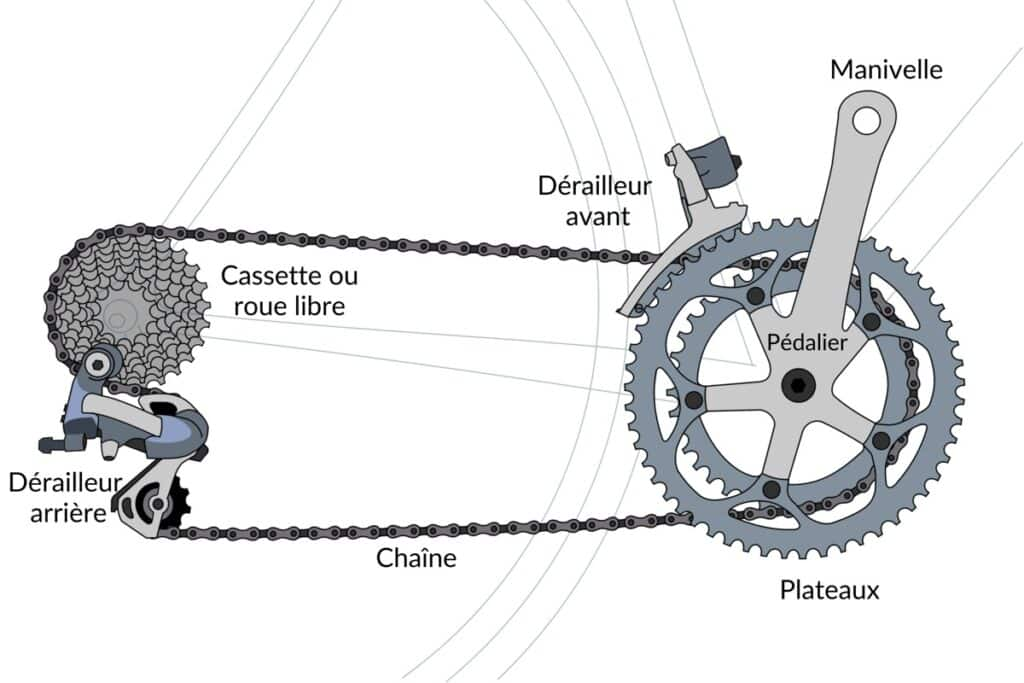
\includegraphics[width=0.4\linewidth]{5x2-inegalite-triangulaire/velo.jpg}
\end{figure} 

Soyons réaliste, vous avez plus de chance de croiser votre professeur en vélo. Équipé d'un rutilant VTT Décath et de gros mollets, il grimpe la côte en petit plateau et grand pignon. Quand il réalise un tour entier avec le pédalier, la roue arrière fait un quart de tour. Il compte 146 tours de pédalier. 

\begin{enumerate}
  \item[1.] Combien de tours la roue a-t-elle effectué ?
  \item[2.] La roue a un rayon de 58cm. Calculer la distance parcourue. \\
    Rappel : Longueur du contour d'un cercle : $P = 2 \times \Pi \times Rayon$.   
\end{enumerate}


\end{document}